%% Dokumenteinstellungen
\documentclass[
    type=Prakikumsbericht,
    status=draft, % Ändern zu "final" für die Abgabeversion
    language=german, % oder: "english"
    bibengine=bibtex,
]{unibwm-inf-thesis}

\usepackage{textcomp}
\usepackage{verbatim}
\usepackage{listings}
\bibliographystyle{apalike-german}
\usepackage{url}
\usepackage{subcaption}
\newcommand{\todo}[1]{\textbf{TODO: #1}}
\setvalue{title}{Qualitätssicherung im Schaltanlagenbau: Konzeption und Implementierung DPP}
\setvalue{author}{Joel Temiz}
\setvalue{matrnr}{1196670}

\setvalue{examiner}{Prof. Dr. Ulrike Lechner}
\setvalue{advisor}{Hptm Lisa Verlande}
\setvalue{advisorlabel}{Betreuerin}
\setvalue{seminartitle}{Praxisprojekt}
\setvalue{seminarcontext}{Sommertrimester 2022}
\setvalue{deadline}{30.09.2022}
\usepackage{amsmath}
\usepackage{nameref}
\usepackage[printonlyused]{acronym}
\begin{document}
    \tableofcontents

    \mainmatter

    \chapter{Einleitung und Motivation}
    Die Idee der Fließbandfertigung geht auf das Ende des 19. Jahrhunderts zurück.
    Zu dieser Zeit wurde in den Schlachthöfen Chicagos das erste Mal ein industrieller Wertschöpfungsprozess im Fließband-Verfahren erstellt.
    Mit der Idee, dass sich eine Arbeitskraft während der gesamten Schicht nur einem Arbeitsschritt der gesamten Wertschöpfungskette widmet und das Produkt sich nach Abschluss zur nächsten Arbeitskraft bewegt, gelang es den Fertigungsprozess um ein Vielfaches zu optimieren~\citep{Pretting2006}.
    Dieselbe Absicht verfolgt seit mehreren Jahren der Fräsmaschinenhersteller DMG MORI AG.
    Dieser hat zur Optimierung der Durchlaufzeiten im Produktionswerk Pfronten im Allgäu die Excellence Factory ins Leben gerufen, die angelehnt an die Automobilindustrie in der Fertigung eine Fließbandfertigung vorsieht~\citep{DMG2020}.

    Diese Umstellung führte zu erhöhten Anforderungen an die Lieferanten des Fräsmaschinenherstellers.
    Vor allem in der Fließband-Produktion wirken sich fehlerhafte Baugruppen negativ auf die Durchlaufzeit aus.
    Im Falle eines Defekts muss das gesamte Produkt aus dem Kreislauf entnommen werden und in der Nacharbeitungszone überarbeitet werden.
    Um den gestiegenen Anforderungen seines Hauptkunden DMG MORI gerecht werden zu können, strebt der Schaltanlagenhersteller Besel und Schwäller GmbH in Füssen an, die Einführung eines Qualitätssicherungssystems für die Schaltanlagen an.

    Im Zuge dieses Praxisprojekts sollte hierfür der erste Stein gesetzt werden.
    Dazu sollte im ersten Schritt die Erarbeitung eines groben Gesamtkonzepts der Individualsoftware \ac{DPP} erfolgen.
    Zur Erarbeitung des Konzepts sollen hierfür die bereits gesammelten Ideen und Anforderungen an das System geordnet und strukturiert werden.
    Aufbauend darauf sollte erörtert werden, wie das System zur besseren Wartung und Weiterentwicklung aufgebaut sein kann.

    Als Schwerpunkt des Praxisprojekts sollte darauffolgend mit der Implementierung begonnen werden.
    Hierbei wurde sich auf die Umsetzung der digitalen Maschinenakte und des Moduls \textit{\ac{DPP} Visual} beschränkt.

    \chapter{Gesamtkonzept von \ac{DPP} und Einordnung in Fertigungsprozess}
    Zur Umsetzung eines betrieblichen Anwendungssystems muss im ersten Schritt eine Konzeption erfolgen, die darstellt,
    wie die Anwendung gestaltet sein kann, um das gewünschte Ziel zu erfüllen.
    Die Anfertigung der Konzeption erfolgte stets in enger Zusammenarbeit mit dem Product Owner, bzw. dem Praxispartner.
    Hierfür wurden wöchentlich im Meeting die Fortschritte am Projekt dargestellt, sowie die geplanten Vorhaben der kommenden Woche vorgestellt.

    \section{Anforderungen}
    In Rücksprache mit dem Praxispartner, wurden einerseits die Ziele des Systems \ac{DPP} herausgearbeitet.

    Andererseits wurden einzelne Anforderungen konkretisiert, die dazu dienen sollen, das Ziel zu erfüllen.
    Das Hauptziel des Anwendungssystems \ac{DPP} ist die Minimierung von fehlerhaften Schaltanlagen.
    Als Anforderung wurden hierbei eine maximale Fehlerquote von 3\% genannt.

    Um dieser Anforderung gerecht werden zu können, stellt sich der Praxispartner verschiedene Leistungen vor.
    Diese sind einerseits dem Prüfprozess zuordenbar, andererseits soll bereits die Entstehung von Fehlern vermieden
    werden, indem die Monteure während der Produktion unterstützt werden.

    \subsection{Digitale Maschinenakte}\label{subsec:digitale-maschinenakte}
    Zur Verwirklichung des Systems ist es notwendig, die physische Entität des Schaltschranks um eine zusätzliche,
    virtuelle Dimension zu erweitern.
    Diese virtuelle Komponente lässt sich als eine digitale Maschinenakte beschreiben und begleitet das Produkt vom
    Auftragseingang über die Produktion bis hin zur Qualitätssicherung.
    Weiter wäre es denkbar, diese auch nach der Auslieferung noch besteht, um Wartungs- und Reparaturvorgänge
    dokumentieren zu können.
    Sie soll dem jeweiligen Schaltschrank über seine Seriennummer eindeutig zuordenbar sein, sodass sie dauerhaft
    aktualisiert werden kann und auch Informationen aus ihr hervorgehen können.
    Beispielsweise soll sie es im Zuge des kontinuierlichen Verbesserungsprozesses ermöglichen, bei einem in der
    Qualitätssicherung erkannten Mangel auf einen vorhergehenden Montageschritt verweisen zu können.
    Einträge der digitalen Maschinenakte, die im Laufe der Produktion und Qualitätssicherung notwendig sind, sind unter
    anderem:
    \begin{itemize}
        \item CAD-Modell des Schaltschranks
        \item Montagepläne
        \item Schaltpläne
        \item Stücklisten
        \item Simulation der zugehörigen Maschine
    \end{itemize}



    \subsection{Kontinierliche technische Prüfung}\label{subsec:kontinierliche-technische-prufung}
    Die erste Leistung ist die \ac{ktP} der Schaltschränke durch Simulation.
    Ziel der \ac{ktP} ist die Auflösung der isolierten Produktion von Schaltschrank und Mechanik.
    Hierbei soll die Maschine, für die die Schaltanlage gebaut wird, durch ein System simuliert werden.
    Der zu produzierende Schaltschrank wird hierzu während der Produktion mit einem Simulationssystem verbunden, das die Logik der zugehörigen Maschine dauerhaft simuliert.
    Liegt ein technischer Fehler im Schaltschrank vor, würde dieser Fehler direkt im Zuge der Produktion auffallen, sodass bereits vor der Auslieferung auf den Defekt reagiert werden kann.
    Weiter soll das System den derzeitigen Arbeitsfortschritt kennen, um ausschließlich die bisher funktionierenden Baugruppen zu prüfen und folglich realistische Fehlereinschätzungen zu liefern.

    Ein reduzierter Prototyp für Software und Hardware der \ac{ktP} existiert bereits.
    Diese ist bislang jedoch lediglich für eine Version eines Produkts ausgelegt und agiert ohne Kommunikation zu anderen Systemen.
    Die Herausforderung hierbei liegt darin, die \ac{ktP} automatisiert und generisch für jeden Schaltschrank zu ermöglichen.
    Dazu muss die, in der Maschinenakte hinterlegte Simulation durch das System selbstständig aktualisiert werden.
    Da für diese die Logik der Schaltpläne notwendig ist, werden Schnittstellen zu dem Schaltplan-CAD-System benötigt.
    Eine Rücksprache mit dem Unternehmen EPLAN hat zu Beginn des Projektes stattgefunden.
    Dieses sicherte zu, zum Zwecke der Umsetzung der Schnittstellen bestmöglich zu unterstützen.

    \subsection{Visuelle Prüfung}\label{subsec:visuelle-prufung}
    Die visuelle Prüfung soll durch Kamera-gestützte Sensorik erfolgen.
    In der Qualitätssicherung soll dabei lediglich ein oder mehrere Fotos des jeweiligen Schaltschranks gemacht werden, die in das System geladen werden.
    Das System soll das Bild / die Bilder darauffolgend verarbeiten und auf mehrere Gesichtspunkte prüfen.
    Gesichtspunkte, die vom Product Owner aufgezählt wurden, sind
    \begin{itemize}
        \item Verfügbarkeit der Bauteile: Die Bauteile / Baugruppen, die auf der Stückliste des Schaltplans oder
        CAD-Modells aufgezählt sind, müssen im Schaltschrank verbaut sein
        \item Richtige Position der Bauteile: Die Einbauposition der jeweiligen Bauteile / Baugruppen müssen stets an
        der dafür vorgesehenen Position im Schaltschrank verbaut sein
        \item Optische Beschädigungen: Optische Beschädigungen am Äußeren des Schaltschranks dürfen nicht vorhanden sein
    \end{itemize}


    \subsection{Fehlerfreies Arbeiten}\label{subsec:fehlerfreies-arbeiten}
    Die Funktion \textit{Fehlerfreies Arbeiten} ist in dem Kontext nicht direkt der Qualitätssicherung zuzuweisen.
    Ihr Ziel ist es, den laufenden Produktionsprozess dahingehend zu unterstützen, dass Fehler in der Montage von
    Beginn an vermieden werden.
    Dies soll erreicht werden, indem im Produktionsprozess Technologien eingesetzt werden, die den Monteur schrittweise
    durch die Produktion begleiten und ihm Anweisungen zur Montage der Bauteile / Baugruppen geben.
    Vom Product Owner wurde hier beispielsweise der Einsatz von AR-Brillen genannt, die dem Monteur bei seiner Arbeit
    die vorgesehene Position eines Bauteils einblendet, bzw. das Bauteil an der vorgesehenen Position visuell simuliert.
    Als weitere Technologie wurde Cobotik genannt.
    Ein Anwendungsbeispiel hierfür könnte das automatische Ablängen der Kabelkanäle oder Hutschienen sein.
    Außerdem ist eine häufige Fehlerquelle das falsche Anzugsdrehmoment von Schrauben im Schaltschrank.
    Dem kann durch elektronische Drehmomentschlüssel mit voreingestelltem Drehmoment vorgesorgt werden.


    \section{Architektur von DPP}
    Nach Betrachtung der Anforderungen ist erkennbar, dass die drei Funktionen \textit{Kontinuierliche Technische
    Prüfung}, \textit{Visuelle Prüfung} und \textit{Fehlerfreies Arbeiten} prinzipiell unabhängig voneinander interagieren.
    Allesamt benötigen sie lediglich die Daten der digitalen Maschinenakte.
    Da keine paarweise Assoziation zwischen den Funktionen notwendig ist, würde es sich anbieten, sie als autarke Services
    bereitzustellen.
    Diese müssten dann lediglich zum Erhalt der Daten mit der digitalen Maschinenakte und zur Integration in den
    Fertigungsprozess mit dem Client gekoppelt werden.
    Denkbar wäre es folglich, die einzelnen Funktionen als eigenständige Module oder Services umzusetzen.
    Dadurch wäre einerseits die Wartungsfähigkeit erleichtert, da die Änderung in einem Modul keine Auswirkungen auf die anderen hätte.
    Weiter würde damit die Wiederverwendbarkeit und Erweiterbarkeit gesteigert werden.
    Entscheidet sich der Schaltanlagenhersteller, die einzelne Funktionen des Systems auch in anderen Werken einzusetzen, wird lediglich die digitale Maschinenakte benötigt.
    Die restlichen Module könnten folglich frei und unabhängig miteinander kombiniert werden.\\

    Die Umsetzung eines der genannten Module wird im folgenden Kapitel beschrieben.


    \chapter{Implementierung \textit{Visuelle Prüfung}}
    Die Umsetzung des Moduls \textit{Visuelle Prüfung} erfolgte in mehreren Schritten.
    Das Modul wurde in diesem Zuge zu \ac{DPP} Visual umbenannt.

    \section{Machbarkeitsanalyse}
    Als ersten Schritt wurde hierfür eine grobe Machbarkeitsanalyse durchgeführt, anhand der ermittelt werden sollte,
    ob die visuelle Identifizierung der Bauteile ohne bauliche Ergänzungen, wie QR- / Bar-Codes auf den Komponenten erfolgen kann.
    Dazu wurde primär Literatur-Recherche betrieben.
    Die Recherche fächerte sich dabei auf in wissenschaftliche Arbeiten, die sich mit der automatisierten Identifikation von Bildinhalten beschäftigen.
    Beispiele hierfür sind die Identifikation von Unterschriften~\citep{Munich2003} oder andere untergeordnete Komponenten, wie Schrauben~\citep{Lehr2019}.

    \section{Einarbeitung}
    Nachdem festgestellt werden konnte, dass die Objekterkennung und Identifikation von augenscheinlich ähnlichen Objekten möglich ist, wurde sich in die Bildverarbeitungstools eingearbeitet.
    Durch den Praxispartner konnten hierbei Libraries wie OpenCV, oder Pillow genannt werden.
    Diese verfügen zu der umfangreichen Funktionspalette eine vollständige Dokumentation, die bei der Umsetzung unterstützt~\citep{OpenCV2022}.

    In der Einarbeitung in die Tools konnte auf verschiedene Ansätze gestoßen werden, auf die im Folgenden eingegangen wird.

    \subsection{Template Matching}
    Als erster Ansatz wurde das Template-Matching näher betrachtet.
    Dieses hat das Ziel einen Bild in einem anderen Bild zu finden und zurückzugeben~\cite{CV2TemplateMatching2022}.
    Die Attraktivität des Ansatzes ergibt sich aus dem Umfang der Implementierung, die in weniger als 20 Zeilen umsetzen lässt.
    Jedoch muss für ein positives Ergebnis das Request-Bild zwingend eine Teilmenge des Hauptbildes sein, wobei sich maximal die Pixeldichte der Bilder unterscheiden darf.
    Da dies ein eindeutiges Ausschlusskriterium darstellt, wurde die Weiterverfolgung des Ansatzes für die Umsetzung von DPP-Visual früh eingestellt.

    \subsection{Feature-Matching}
    Das Feature-Matching stellte hierbei eine vielversprechendere Variante für die Objekterkennung elektronischer Komponenten dar.
    Dieses beschreibt den Vorgang, dass anhand eines ausgewählten Algorithmus markante Punkte (= \ac{KP}) in einem Bild erhoben werden.
    Zu jedem \ac{KP} wird anschließend eine Beschreibung in Hinblick auf die Daten seiner umliegenden Pixel erstellt.
    Diese Beschreibung ermöglicht den Vergleich zweier Bilder, indem die \ac{KP} auf Ähnlichkeiten geprüft werden.\cite{CV2FeatureMathing2022}

    Sowohl für den Prozess der Analyse der \acp{KP} im Bild, als auch der Überprüfung der Ähnlichkeit (= Matching) zwischen Request-Bild und der Vorlage
    existieren verschiedene Algorithmen, die einen Einfluss auf die Ergebnisse haben.
    Bei der Analyse der \acp{KP} stehen unter anderem die Algorithmen
    \begin{itemize}
        \item \ac{SIFT}
        \item \ac{SURF}
        \item \ac{ORB}
    \end{itemize}
    zur Verfügung.
    Die verschiedenen Algorithmen unterscheiden sich einerseits in ihrer Komplexität und damit auch in ihrer Geschwindigkeit, sowie in dem Umfang ihrer Ergebnismenge.
    Einen Überblick über die Vor- und Nachteile liefern \citet{Karami2017}.
    Zudem wurde die Auswahl empirisch getestet, indem eine Teilmenge der Algorithmen umgesetzt und ihr Ergebnis mit einem Test-Datensatz überprüft wurden.
    Während der \ac{ORB}-Algorithmus die \acp{KP} am schnellsten analysierte, gab dieser lediglich die Hälfte der \acp{KP} des \ac{SIFT}-Algorithmus zurück.
    Dahingegen war der \ac{SURF}-Algorithmus langsamer, als der \ac{SIFT} und lieferte eine vergleichbare Menge an \acp{KP} zurück.
    Da die Durchlaufzeit der Anwendung eine geringere Priorität als die Zuverlässigkeit der Erkennung besitzt, fiel die Entscheidung auf den \ac{SIFT}-Algorithmus.

    Das Matching hat die Aufgabe, die Beschreibungen zweiter \acp{KP} miteinander zu vergleichen und festzustellen, ob sie ähnlich zueinander sind.
    Hierbei gibt es ebenso mehrere Ansätze, von denen vor allem zwei in der Dokumentation von OpenCV vertreten sind:
    \begin{itemize}
        \item BruteForce
        \item \ac{FLANN}-Based
    \end{itemize}

    Das BruteForce-Verfahren ermittelt hierbei die $L_{2}$-Norm von jedem \ac{KP} zu jedem \ac{KP}, wodurch sich die Menge der Rechenschritte durch die Funktion
\begin{center}
    $f(x) = n * m,$ \\
    $wobei~n= Menge~der~ermittelten~Keypoints~im~Requestbild;$\\
    $m = Menge~der~Key-Points~im~Template-Bild$\\
\end{center}
    beschreiben lässt.
    Die Komplexitätsstufe nach Landau-Notation beträgt im worst case folglich $O(n^{2})$.

    Einen weniger komplexen Ansatz soll hierbei der \ac{FLANN}-based Matching-Algorithmus liefern.
    Im \ac{FLANN} Algorithmus soll der \textit{approximate nearest neighbor} ermittelt werden, der nicht zwangsläufig der nächste Nachbar (entspricht dem Punkt mit der größten Ähnlichkeit) sein muss,
    ihm jedoch sehr nahekommt.
    Zur Ermittlung des \textit{aproximate nearest neighbors} wird der Datensatz in einen KD-Tree überführt, der es erlaubt, dass sich die Menge der zu vergleichenden \acp{KP} sich auf ein KD-Tree-Feld begrenzt.
    Unter der Annahme einer gleichmäßigen Verteilung aller Punkte über die KD-Tree-Felder würde die sich die Anzahl der Rechenschritte somit auf
    \begin{center}
        $f(x) = (m*n) / k, $ \\
        $wobei~n= Menge~der~ermittelten~Keypoints~im~Requestbild;$\\
        $m = Menge~der~Key-Points~im~Template-Bild$\\
        $k = Menge~der~KD-Tree-Felder$\\
    \end{center}
    begrenzen.

    In einem direkten Vergleich mit einem Beispieldatensatz konnte festgestellt werden, dass der \ac{FLANN}-based Matcher nahezu identische Ergebnisse wie der BruteForce-Matcher liefert.
    In Kombination mit der Ersparnis von Rechenleistung fiel die Entscheidung somit auf den \ac{FLANN}-based Matcher.\\

    Der Rückgabewert der Matching-Methoden beinhaltet einen Array von Positionen, die darstellen, wo im Request-Bild Übereinstimmungen mit dem Vorlage-Bild gefunden werden konnten.
    Da diese Übereinstimmungen auch fehlerhafte Positionen beinhalten, die sich über das ganze Bild verstreuen können, musste im darauffolgenden Schritt eine Methode erarbeitet werden, um Fehlerdaten zu erkennen.
    Ein Beispiel für eine Sammlung unbereinigter Matches ist \autoref{fig:plottedMatches} zu entnehmen.
    \begin{figure}[b]
        \centering
        \begin{subfigure}{.5\textwidth}
            \centering
            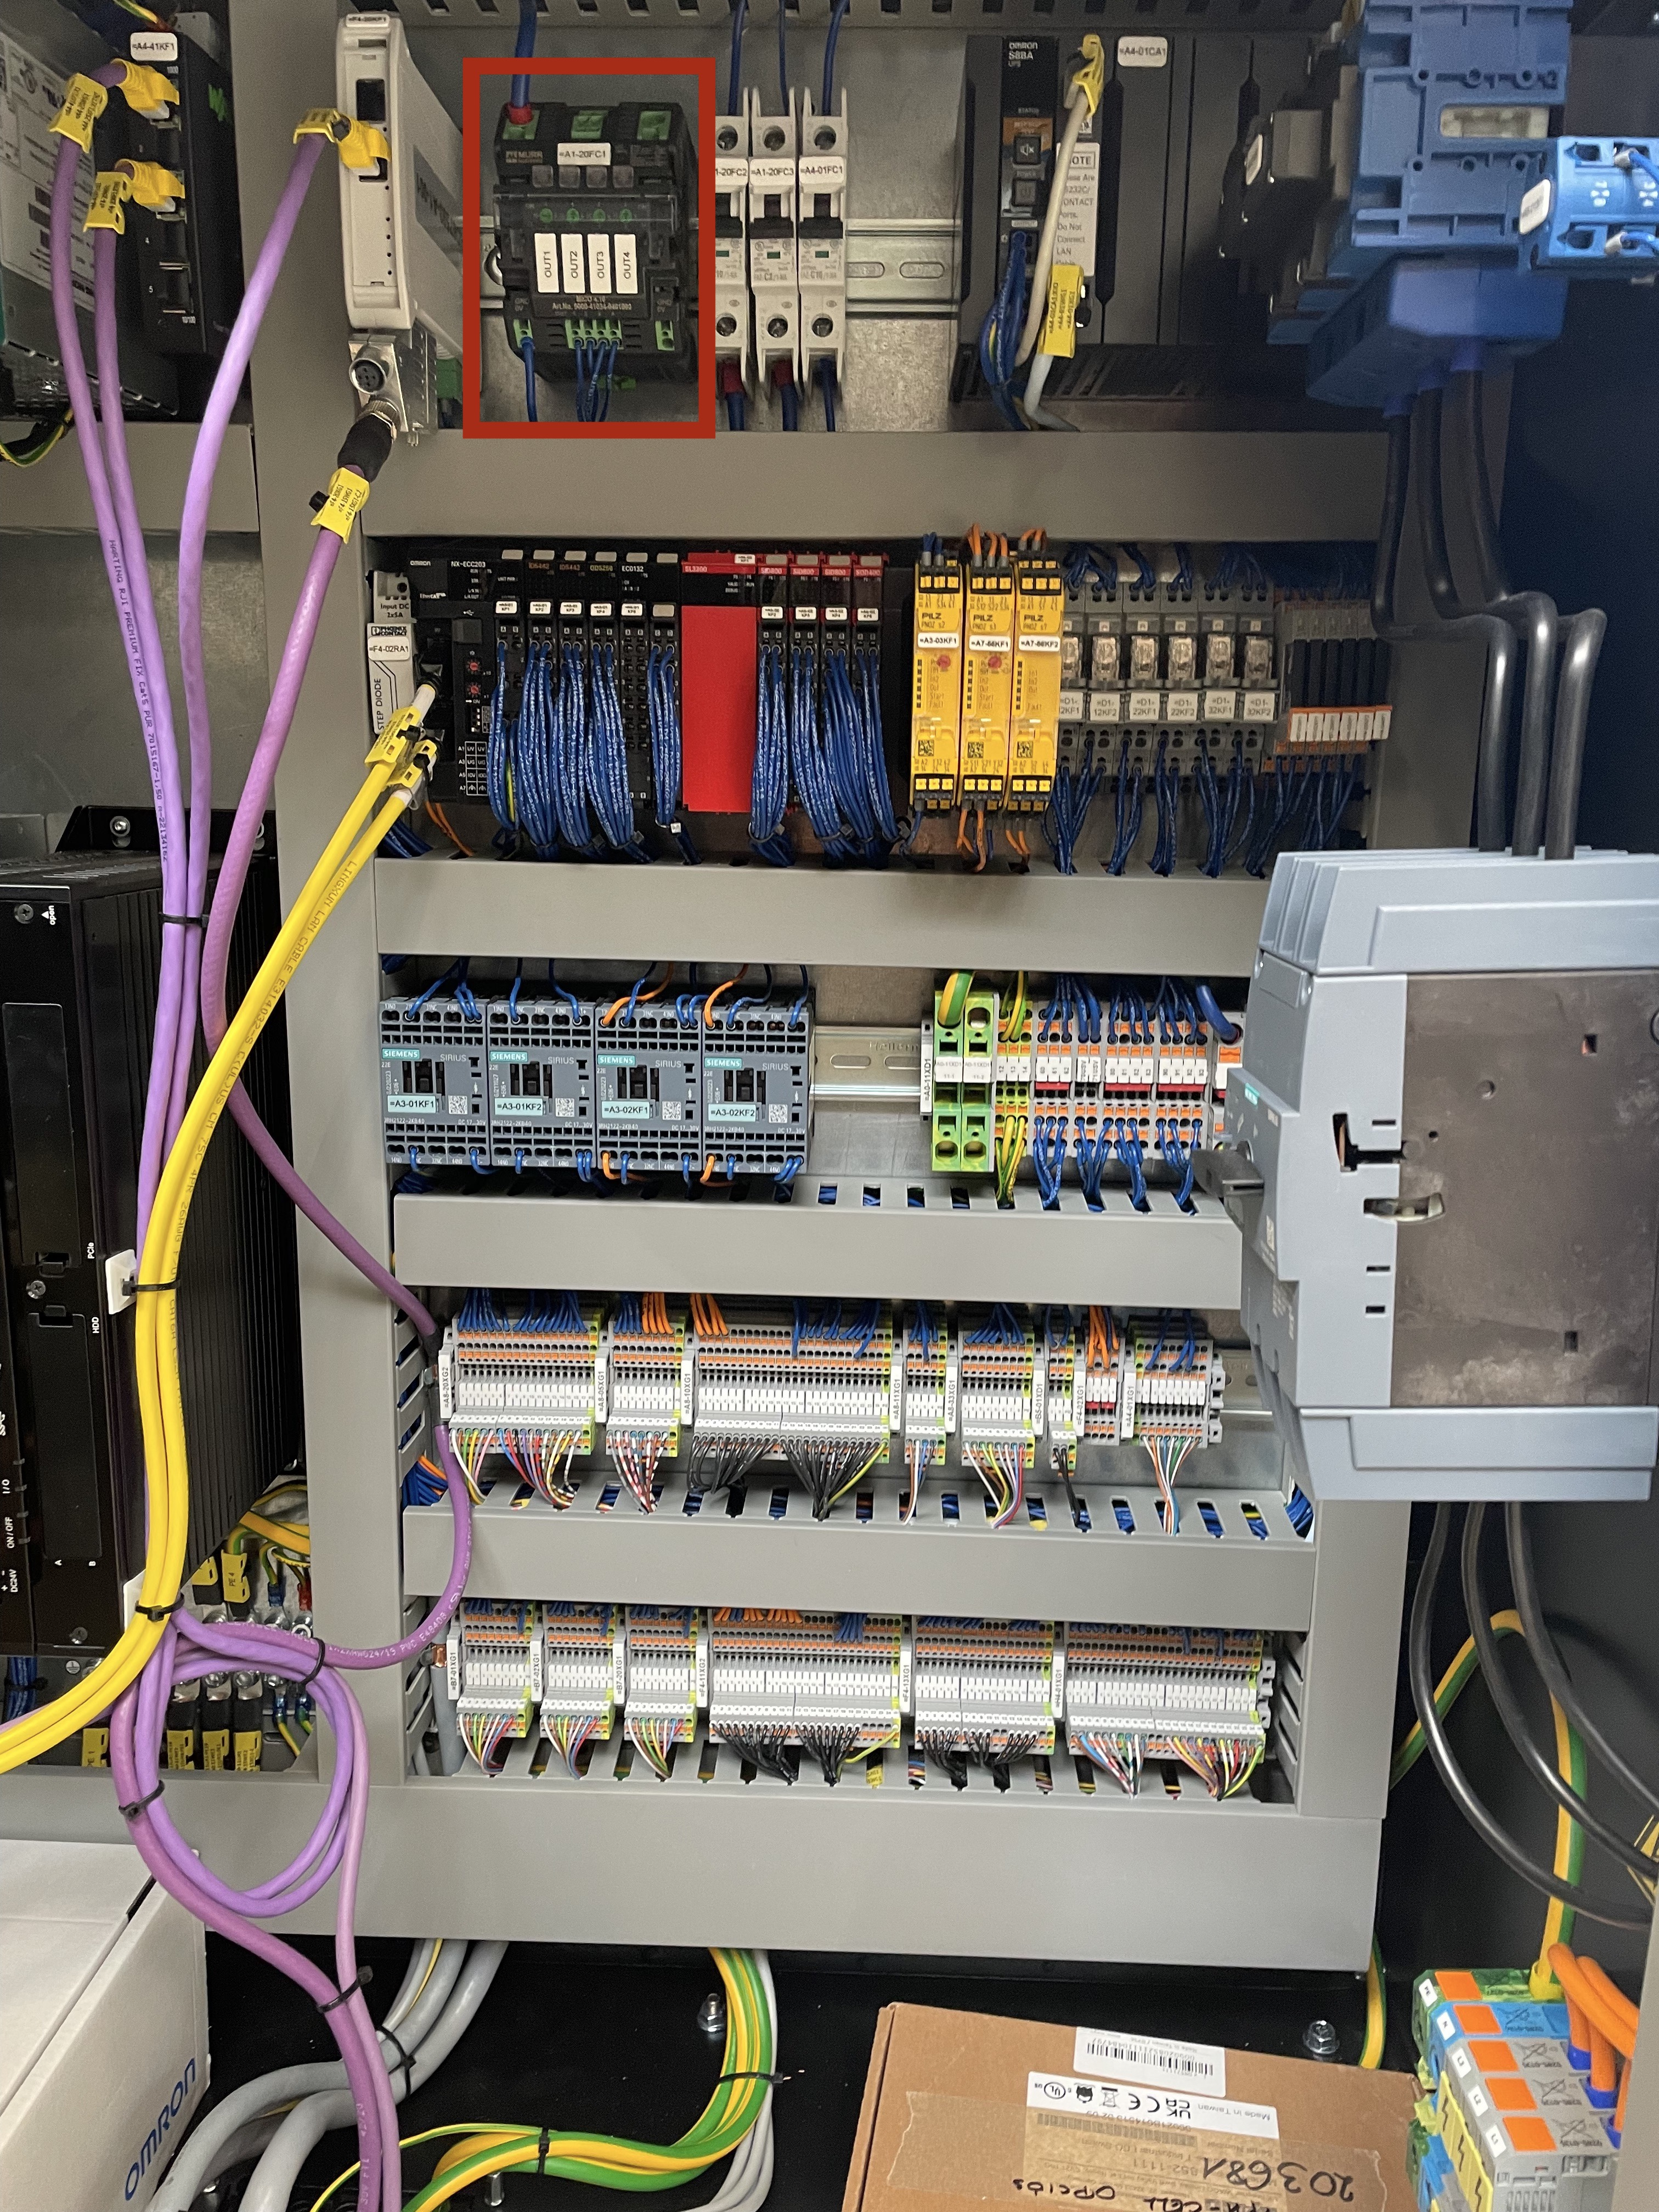
\includegraphics[width=1.0\textwidth]{images/Request_image}
            \caption{Request-Bild mit gesuchtem Objekt rot umrandet}
            \label{fig:sub1}
        \end{subfigure}%
        \begin{subfigure}{0.5\textwidth}
            \centering
            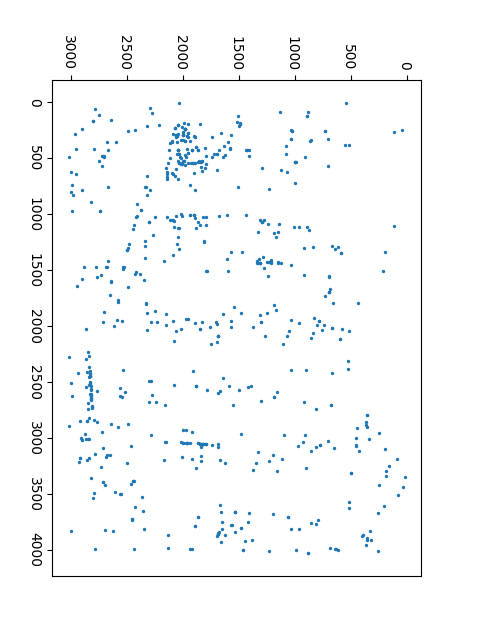
\includegraphics[width=1.0\textwidth]{images/Request_plot}
            \caption{Gefundene Übereinstimmungen im Bild}
            \label{fig:sub3}
        \end{subfigure}
        \caption{Ansicht der gefundenen Matches zwischen Request-Bild und Vorlage}
        \label{fig:plottedMatches}
    \end{figure}

    Bei Betrachtung der Verteilung der Matching-Positionen im Request-Bild lässt sich erkennen, dass sich die Punkte nicht gleichermaßen über das Bild verteilen, sondern sich meist ein Punkt-Zentrum mit höherer Punkte-Konzentration bildet.
    Beim Abgleich dieses Zentrums mit dem Request-Bild kann festgestellt werden, dass sich das gesuchte Objekt meistens in dem ermittelten Zentrum befindet.
    Die Punkte, die außerhalb des Zentrums liegen, sind somit fehlerhafte Daten oder Ausreißer (= Outlier).
    Zur generischen Ermittlung der Outlier wurden verschiedene Ansätze erarbeitet.

    \subsection{Bereinigtes KMeans-Cluster}
    Zu Beginn wurde für die Ermittlung des Punktezentrums und die Ausreißer ein Clustering des Datensatzes mittels KMeans durchgeführt.
    Da KMeans jeden Punkt des Datensatzes einem Cluster zuordnet, werden auch Outlier in das Cluster aufgenommen,
    sofern ihre euklidische Distanz zum Cluster-Schwerpunkts (= Centroid) des korrekten Clusters geringer ist, als die zu den restlichen Clustern.
    Das Ergebnis ist, dass es zum einen mehrere Cluster gibt, die im weiteren Verlauf als gesuchten Bildausschnitt gewertet werden können.
    Zum anderen bewirken Datenpunkte, die stark von ihrem Cluster-Centroid abweichen, dass sich die Außenkanten des Bildausschnitts nach außen hin ausweiten.
    Eine Überlegung zur Beseitigung dieser Datenpunkte war die Minimierung des Clusters auf seine Standardabweichung.
    Hierzu wurde die Standardabweichung in beiden Dimensionen ermittelt, wodurch sich ein Kreis mit dem Radius $\sigma$ um den Centroid des Clusters bildete.
    Im darauffolgenden Schritt wurden alle Punkte, die Element des Clusters sind und sich außerhalb dieses Kreises befinden, eliminiert.

    Aus diesem Ansatz heraus ergaben sich zwei Fragen:
    \begin{itemize}
        \item Welches der k Cluster repräsentiert den korrekten Bildausschnitt?
        \item Welcher ist der korrekte Schwellenwert, um Outlier zu definieren?
    \end{itemize}

    Für die Frage des Outlier-Schwellenwerts können alternative Ansätze hierbei verfolgt werden.
    Als Beispiele kann die \textit{Depth-Based Outlier detection} oder die \textit{Extreme Value Analysis} genannt werden, die zielführendere Ergebnisse als die Ermittlung per Standardabweichung liefern können.
    Dennoch bleibt dann weiterhin die Frage, welches der Cluster den gesuchten Bildausschnitt korrekt repräsentiert.
    Weder das Cluster mit der größten Datenpunkt-Dichte, noch das Cluster mit der größten Datenpunkt-Anzahl kann in jedem Fall eindeutig das Bild identifizieren.

    Ein weiterer Ansatz, der dazu für kurze Zeit verfolgt wurde, war die Identifizierung über Farbhistogramme.
    Hierbei wurden Farbhistogramme aller geclusterten Bildausschnitte, sowie dem Vorlage-Bild erstellt.
    Farbhistogramme stellen die Verteilung der Graustufen-Werte anhand eines 2D-Graphen dar.
    Dabei repräsentiert die x-Achse die Graustufe (Wert zwischen 0 und 255), und die y-Achse die Anzahl an Pixeln, die diesen Farbwert besitzen.

    Die Farbhistogramme der geclusterten Bildausschnitte wurden im Anschluss auf Ähnlichkeit mit dem Farbhistogramm des Template-Bilds verglichen.
    Die Ermittlung der Ähnlichkeit erfolgte mittels vierer Algorithmen (Korrelation, Chi-Quadrat, Intersection und Hellinger), die im Anschluss miteinander korreliert wurden.
    Als korrekter Bildausschnitt wurde derjenige identifiziert, dessen Ähnlichkeit am höchsten war.

    Das Ergebnis des Farbhistogramm-Ansatzes wurde mittels eines Test-Datensatzes geprüft.
    Dabei wurden hohe Fehlerquoten festgestellt.
    Es ließ sich daraus schließen, dass die Identifizierung des korrekten Clusters über KMeans nicht ohne Weiteres möglich ist.
    Aus diesem Grund wurde im weiteren Verlauf auf einen alternativen Clustering-Algorithmus umgestiegen.

    \subsection{Density-Based Spatial Clustering of Applications with Noise}\label{subsec:dbscan}
    Der \ac{DBSCAN} Clustering-Algorithmus hat im Vergleich zu Algorithmen wie KMeans entscheidende Unterschiede, die für die Umsetzung der Objekterkennung vorteilhaft sind.
    Einer der wichtigsten Vorteile ist hierbei die Basis der Cluster-Ermittlung.
    Diese geschieht in \ac{DBSCAN} über die Dichte des Clusters, anstatt über die euklidische Distanz zum Centroid.
    Konkreter wird, ein Datenpunkt dem Cluster seines nächsten Nachbarn zugerechnet.
    Die Zurechnung erfolgt jedoch nur dann, wenn die Konditionen der Übergabeparameter erfüllt sind.

    Als eine dieser Konditionen gilt der Parameter \textit{min-samples}, die Toleranz für Rauschen beschreibt.
    Eine Sammlung von Datenpunkten wird dann als Rauschen betitelt, wenn ihre Anzahl zu gering ist, um ein eigenes Cluster zu bilden.
    Datenpunkte sollen folglich als Rauschen markiert werden, wenn ihre Anzahl \textit{min-samples} nicht übersteigt.
    Sie gelten im Anschluss als kein eigenes Cluster.

    Der Übergabeparameter \textit{eps} dahingegen beschreibt die maximale Distanz zu seinem nächsten Nachbarn, bis ein Datenpunkt als Outlier bezeichnet wird.
    Er wird somit keinem Cluster zugeordnet und wird gleich wie das Rauschen im weiteren Verlauf nicht beachtet~\citep{Bedre2022}.
    \autoref{tab:matrix-dbscan} zeigt die Auswirkung der Wahl der Übergabeparameter auf das Clustering-Ergebnis bei \ac{DBSCAN}.
    \begin{table}[h]
        \centering
        \begin{tabular}{c | c | c}
            & Epsilon groß & Epsilon klein \\ \hline
            min-samples groß & wenige sehr große Cluster & große Anzahl an Outlier\\ \hline
            min-samples klein & viele kleine Cluster, kaum Outlier & viele kleine Cluster, wenig Outlier
        \end{tabular}
        \caption{Auswirkungen der Parameter-Wahl \textit{min-samples} und \textit{Epsilon} auf \ac{DBSCAN}-Cluster}
        \label{tab:matrix-dbscan}
    \end{table}

    Wie die Funktionsweise von \ac{DBSCAN} zeigt, ist die Zahl der Cluster im Gegensatz zu den meisten anderen Cluster-Algorithmen variabel.
    Diese Eigenschaft ist für die Implementierung der Objekterkennung dahingehend vorteilhaft, dass keine Cluster \glqq erzwungen\grqq{} werden.
    Sollte ein gesuchtes Objekt in dem Request-Bild nicht vorhanden sein, würde das Clustering alle Datenpunkte als Rauschen oder Outlier kennzeichnen, wodurch kein Cluster entstünde.

    Anhand eines Test-Datensatzes wurde versucht, diese Vorteile in der Praxis zu bestätigen.
    Nachdem das Clustering des Test-Datensatzes durchwegs positiv war, wurde sich auf den \ac{DBSCAN}-Algorithmus für das Clustering entschieden.

    
    \section{Konzeption}
    Nachdem sich in die einzelnen Elemente der Objekterkennung eingearbeitet wurde, begann die Konzeption des Moduls \ac{DPP} Visual.
    Dazu wurde im ersten Schritt eine Programmiersprache gewählt, die den Anforderungen an das System gerecht werden kann.
    Im nächsten Schritt wurde eine grobe Konzeption des Tools erstellt, anhand die es ermöglichen sollte, strukturiert an das Problem heranzugehen.

    \subsection{Programmiersprache}
    Im Zuge der Implementierung des Moduls DPP Visual werden zahlreiche Methoden der Bildverarbeitung und des
    Computer-Visions benötigt.
    Zudem werden Algorithmen zum Umgang mit großen Datenmengen, wie Clustering, verwendet.
    Eine weitere Anforderung für den weiteren Verlauf ist die Unterstützung der Intel RealSense SDK, die benötigt werden kann,
    um Aufnahmen der 3D-Kamera zu verarbeiten.

    Eine Programmiersprache, die diese Anforderungen allesamt erfüllt, ist Python.
    Diese bietet neben der Unterstützung der Intel RealSense SDK zahlreiche Libraries wie \textit{OpenCV, Numpy, Pandas, Pillow} etc., die bei der Lösung von Problemen in der Mathematik sowie der Computer-Vision unterstützen.

    Diese Libraries können mit vergleichsweise geringem Aufwand über den Pip-Installer in die Anwendung integriert
    werden, sodass der Funktionsumfang deutlich erweitert werden kann.

    Für die Umsetzung der Testumgebung wurde zusätzlich das Python-basierte Framework \textit{Flask} mit der
    Template-Engine \textit{Jinja} herangezogen.
    Diese Kombination ermöglicht es eine webbasierte Oberfläche umzusetzen, die die Nutzung mit einem mobilen Endgerät
    (Tablet, Smartphone) möglich macht und somit sowohl in der Entwicklungsphase, als auch in der späteren Verwendung eine leicht bedienbare Benutzerschnittstelle liefert.

    \subsection{Aufbau des Tools} \label{subsec:aufbau-des-tools}
    Der Aufbau des Tools erfolgte nach dem Factory-Pattern (Vgl.~\citep{FlaskDevelopero.J.}).
    Unter Vernachlässigung der App-Factory Klassen und Methoden gliederte sich der Aufbau in die View und das Backend.
    Bei der Implementierung der View wurden zum einen die tatsächliche Benutzeroberfläche in der Auszeichnungssprache
    HTML mit der Template-Engine \textit{Jinja} und JavaScript erstellt.
    Diese war für die Entgegennahme der Benutzerinteraktionen und die Darstellung der Inhalte verantwortlich.
    Zum anderen wurde zusätzlich eine View-Model-Schicht hinzugenommen, die als harmonisierende Schicht zwischen
    Frontend und Backend zuständig ist.
    Diese Schicht wurde in Python-Flask realisiert, das es ermöglicht, über Flask-charakteristische Decorator wie
    \textit{@app.route} URLs zur Verfügung zu stellen, über die Methoden aufgerufen werden können.

    Im Backend wurde dahingegen die Logik der Objekterkennung, sowie die Schnittstellen zur virtuellen Maschinenakte realisiert.
    Das Logik-Element teilt sich auf in die Clustering-Logik und die Computer-Vision-Logik, für die jeweils eigene
    Skripte angelegt wurden, die aus dem View-Model heraus erreichbar sind.

    \section{Umsetzung}
    Im folgenden Kapitel wird die letztendliche Umsetzung des Moduls \ac{DPP} Visual beschrieben.
    Der Schwerpunkt liegt hierbei auf der Logik der Objekterkennung.
    Dazu wird im ersten Schritt die Hauptroutine erläutert, die die Anreihung der verschiedenen Methoden beschreibt.
    Im nächsten Schritt werden die beiden Hauptkomponenten der Logik, zu denen das die Ermittlung und das Matching der \acp{KP}, sowie das Clustering zählen, erläutert.

    \subsection{Hauptroutine}
    Die Hauptroutine ist über die Methode \textit{detect\_object(image, template\_collection)} aus dem View-Model heraus erreichbar.
    Darin enthalten ist die gesamte Logik der Objekterkennung, von der Eingabe der Request- und Vorlagebilder bis hin zu den Randpositionen des gesuchten Objekts.

    Die Ausführung der Hauptroutine geschieht, nachdem über die Benutzerschnittstelle das Request-Bild zusammen mit der Seriennummer des zu prüfenden Schaltschranks eingegeben wurde und die Daten zum Schaltschrank aus der digitalen Maschinenakte gelesen wurden.
    Dabei wird die Methode für jede verfügbare und zu testende Komponente im Schaltschrank einmal ausgeführt.
    Als Übergabeparameter erhält die Methode sowohl das Request-Bild, als auch einen Array von Vorlage-Bildern.
    Im ersten Teil der Methode werden die Bilder zu einem, für OpenCV verständlichen Format verändert.
    Im Anschluss erfolgt das Ermitteln der \acp{KP}, indem sowohl das Request-Bild, als auch die Vorlage-Bilder an die Methode \textit{SIFT\_detector()} übergeben werden.
    Die Rückgabe der Methode beinhaltet sowohl eine Sammlung von \acp{KP} des Request-Bilds, als auch einen Array, der für jeden Eintrag die \acp{KP} eines Vorlage-Bilds enthält.

    Diese beiden Rückgabewerte werden darauffolgend in die Matching-Methode \textit{flann\_matcher()} übergeben, die alle Matching-Positionen des Request-Bilds zurückgibt.
    Die erhaltenen Matching-Positionen werden im nächsten Schritt im separierten Skript \textit{cluster\_handler.py} in Cluster überführt.

    Nachdem die Cluster ermittelt wurden, wird das Cluster mit den meisten Datenpunkten ausgewählt.
    Die Positionen der linken oberen, sowie die rechten unteren Ecke repräsentieren das Ergebnis der Methode und werden folglich zurückgegeben.

    \subsection{Key-Detector und -Matcher} \label{subsubsec:Key-Detector-Matcher}
    Ein Kernelement, der eben dargestellten Objekterkennungsroutine ist das Ermitteln und Matchen der \acp{KP} im Bild.
    Bei diesem Prozess wurde für das Ermitteln der \acp{KP} der \ac{SIFT}-Algorithmus und für das Matchen der \ac{FLANN}-based Matcher gewählt.
    Beim Ermitteln der \acp{KP} und der Beschreibungen wird dazu für jedes Bild die Methode \textit{detectAndCompute()} aufgerufen, die als Übergabeparameter, das Bild und die Konfiguration des Detection-Algorithmus erhält.
    Für die Konfiguration wurde in der Umsetzung None als Default-Parameter übergeben.
    Die ermittelten \acp{KP} und ihre Beschreibungen für jedes Bild werden als Tupel in einem Array abgelegt und schließlich zurückgegeben.
    Der \ac{SIFT}-Algorithmus agiert dabei vollends deterministisch.

    Der \ac{FLANN}-based Matcher erhält nach Vollendung der \ac{KP}-Ermittlung alle \acp{KP} und Beschreibungen und vergleicht die einzelnen Vorlage-\acp{KP} mit denen des Request-Bilds.
    Dabei wird über die einzelnen Bilder (repräsentiert durch die \acp{KP} und Beschreibungen) iteriert und für jeden Durchlauf nach Ähnlichkeit zu den \acp{KP} des Request-Bilds gesucht.
    Die Ähnlichkeit wird dabei als $L_{2}$-Norm dargestellt.
    Ein tatsächliches Matching liegt folglich nur vor, wenn gilt $l_{2} > x,~wobei~x~\epsilon~[0; 1]$.
    Eine Ähnlichkeit von 1 würde dabei einer vollkommenen Übereinstimmung entsprechen.

    In der Umsetzung des Tools wurde für die notwendige Ähnlichkeit 0,6 gewählt.
    Die Ermittlung des Werts gelang durch die Analyse der Verteilung der Ähnlichkeiten.
    Die Wahl eines Werts über 0,6 verringerte die Anzahl der Matches dabei um circa 50 \%, wodurch die Wahrscheinlichkeit erhöht wird, dass kein Cluster gebildet werden kann.
    Bei der Wahl eines Werts unter 0,6 stieg wiederum die Fehlerquote massiv an, wodurch die Eliminierung der Outlier und des Rauschens im Cluster erschwert würde.

    Das Ergebnis des Key-Matchers ist ein Array mit Positionen, die darstellen, an welchen Positionen im Bild Übereinstimmungen gefunden werden konnten.
    Diese Positionen werden im Anschluss im Clustering analysiert.

    \subsection{Clustering} \label{subsubsec:clustering}
    Das Clustering ist das zweite Kernelement der Objekterkennung.
    Dieses hat die Aufgabe, die einzelnen Datenpunkte, die Matches darstellen, zu gruppieren und anhand dessen die Bauteilränder im Request-Bild zu ermitteln.
    Dazu werden alle Positionen, die im Request-Bild als Match identifiziert werden konnten als (x, y)-Tupel dargestellt und über den \ac{DBSCAN}-Algorithmus geclustert.
    Der Clustering-Algorithmus \ac{DBSCAN} erhält dafür, wie in \autoref{subsec:dbscan} dargestellt, die zwei Übergabeparameter \textit{Epsilon} und \textit{min-samples}.

    Die Ermittlung der beiden Werte erfolgte in einem iterativen Prozess.
    Dabei wurden ein kleiner Wert für \textit{min-samples} gewählt (hier: $len(matches) / 10 $) und anhand eines Test-Datensatzes die euklidische Distanz jedes Punktes zu seinem nächsten Nachbarn ermittelt.
    Nach der aufsteigender Sortierung der Distanzen und Zeichnung des Graphen bildet sich eine Abwandlung der Exponential-Funktion mit diskreten Werten.

    Der optimale Wert für Epsilon ist dem y-Wert zu entnehmen, an dem der Graph eine gravierende Steigungsänderung besitzt~\citep{Maklin2019}.
    Im nächsten Schritt wurde \textit{min-samples} erhöht und die Zuverlässigkeit des Clusterings beurteilt.
    Diese Schritte wurden wiederholt, bis das Clustering das korrekte Ergebnis lieferte.
    Unter der Konfiguration $eps = 180; ~ min_samples=len(matches) / 4$ lieferte der \ac{DBSCAN}-Algorithmus für den Test-Datensatz die korrekten Outlier, womit der Konfigurationsprozess abgeschlossen war.

    Nachdem die Outlier und Rauschdaten eliminiert werden konnten, bleiben letztlich nur die Werte, die das gesuchte Bauteil repräsentieren.
    Diese werden folglich zurückgegeben.


    \chapter{Evaluation} \label{ch:evaluation}
    Im Zuge der Evaluation sollte die Funktionsweise des entwickelten Systems bewertet werden.
    Hierbei handelt es sich sowohl um die digitalen Maschinenakte, als auch auf das Modul \ac{DPP} Visual.
    Aufgrund der Größe des Projekts und der entsprechend kurzen Zeit des Praktikums erfolgte die Evaluation nur im begrenzten Rahmen.
    Dabei wurde das Modul \ac{DPP} Visual auf die allgemeine Funktionsweise geprüft, sowie auf die Grenzen des Systems und die Dauer des Prüfverfahrens.
    Da das Modul \ac{DPP} Visual die Funktionsweise digitale Maschinenakte mit einschließt, und diese wenig kritische Elemente besitzt, wurde sich bei der Evaluation auf \ac{DPP} Visual beschränkt.

    Das entwickelte Tool wurde auf dem Python3-Development-Server gehostet.
    Dieser lief auf einem Mac Mini mit 3,2 GHz 6-Core Intel Core i7 und 16 GB DDR4 RAM.

    Für die Evaluation wurde in die digitale Maschinenakte der elektronische Schaltplan eines PH-Cell-Schaltschranks eingepflegt.
    Dieser enthält die Stückliste, die alle Komponenten beinhaltet.
    Davon wurden vier Komponenten ausgewählt, für die jeweils 9 bis 17 Bilder der jeweiligen Komponente in die digitale Maschinenakte hinzugefügt wurden (insgesamt 57 Bilder).
    Die kleinste Komponente besitzt dabei eine Größe von 2 x 8 x 8, die größte Komponente 10 x 10 x 10 (Breite x Höhe x Tiefe jeweils in Centimeter).

    Als Nächstes wurde eine Bestellung simuliert, indem eine PH-Cell-Schaltschrank-Instanz im System aufgenommen wurde.

    Zur Prüfung der Funktionsweise und der Grenzen der Objekterkennung wurden mehrere Bilder, von korrekt aufgebauten Schaltschränken als Request-Bilder verwendet.
    Diese wurden mit der Kamera eines Apple iPhone 12s unter guter Belichtung aufgenommen.
    Zur Prüfung der allgemeinen Funktionsweise war die Perspektive der Bilder komplett frontal (10 Bilder).
    Im nächsten Schritt erfolgten die Aufnahmen aus verschiedenen Winkeln bis hin zu + / - 45° (5 Bilder aus positivem, 5 Bilder aus negativem Winkel).
    Weiter wurden Aufnahmen des Schaltschranks gemacht, auf denen einzelne Komponenten nicht vorhanden bzw. zu sehen waren (4 Bilder).

    Zuerst wurden die Frontalaufnahmen zusammen mit der Seriennummer jeweils in die Eingabemaske eingegeben und die Prüfung gestartet.
    Im nächsten Schritt wurde schrittweise der Winkel zum Schaltschrank erhöht.
    Als letztes Testszenario wurden die Aufnahmen verwendet, auf denen Komponenten fehlen.

    \section{Ergebnis}
    Bei den Durchläufen mit Frontalaufnahmen wurden mit wenigen Ausnahmen alle gesuchten Komponenten erkannt.
    Lediglich die Markierung auf den Bildern stimmten dabei jedoch nicht immer mit den Außenkanten der Komponenten überein.
    Bei Frontalaufnahmen auf denen Komponenten unkenntlich gemacht wurden, wurde mit einer Ausnahme immer auf das Fehlen hingewiesen.

    Bei den Aufnahmen aus verschiedenen Winkel stieg die Fehlerquote an.
    Hierbei traten Fehler bereits ab circa + / - 20° auf, sodass teilweise mehrere Komponenten entweder nicht erkannt wurden, oder die Komponenten an falschen Stellen erkannt wurden.

    \textit{False-Negative}-Fälle traten nur in zwei der 25 Tests auf, wohingegen \textit{False-Positiv}-Fälle deutlich häufiger auftraten.
    Dennoch sind die fehlerfreien Durchläufe in den Tests am meisten vertreten.

    Die Durchlaufzeiten für die Testdurchläufe bewegten sich im Bereich zwischen 90 und 180 Sekunden.
    Ein Tracking der Zeiten der Einzelprozesse zeigte, dass ein Großteil der Durchlaufzeit auf die \ac{KP}-Ermittlung mittels \ac{SIFT}-Algorithmus zurückzuführen ist.
    Zu bemängeln ist die Durchlaufzeit Objekterkennung.
    Für die Ermittlung der \acp{KP} eines Bildes werden dabei circa 1,5 bis 2 Sekunden benötigt.
    Bei den hier eingesetzten 57 Bildern werden allein durch diesen Prozess bereits 85 bis 114 Sekunden benötigt.
    Der restliche Teil des Algorithmus spielt in der Durchlaufzeit eine untergeordnete Rolle.

    \section{Limitationen}
    Die Evaluation konnte zeigen, dass das Modul \textit{DPP Visual} grundlegend funktioniert.
    Während Frontalaufnahmen für das System weitestgehend unproblematisch sind, sinkt die Zuverlässigkeit mit ansteigendem Aufnahmewinkel.
    Ab einem Winkel von + / - 20° werden die Ergebnisse zu unzuverlässig, um das Tool sinnvoll einzusetzen.

    Ebenso die Durchlaufzeit ist optimierungsfähig.
    Auch wenn hierfür keine Anforderung durch den Praxispartner definiert wurde, kann eine Durchlaufzeit von mehreren Minuten den Produktionsprozess stören.

    \chapter{Reflektion und Ausblick}
    Wie anhand der Evaluation in \autoref{ch:evaluation} zu sehen ist, leistet das Modul \ac{DPP} Visual für den Anfang gute Ergebnisse.
    Innerhalb der bislang umgesetzten Funktionen ist einerseits die Fehleranfälligkeit bei Aufnahmen außerhalb der Frontalperspektive verbesserungswürdig.
    Ein Ansatz für die Steigerung der Zuverlässigkeit des Systems könnte die eine zusätzliche Kalibrierung der verschiedener Parameter sein.
    Diese sind unter anderem:
    \begin{itemize}
        \item Ähnlichkeit im \ac{FLANN}-based Matcher
        \item Epsilon im \ac{DBSCAN}-Clustering
        \item min-samples im \ac{DBSCAN}-Clustering
        \item Anzahl der Bilder pro Komponente
    \end{itemize}

    Zudem müssen auch diverse Optimierungen vorgenommen werden, um die Durchlaufzeit zu minimieren.
    Eine Anlaufstelle hierbei stellt die \ac{KP}-Ermittlung dar.
    Wie in \autoref{subsubsec:Key-Detector-Matcher} bereits angesprochen, erfolgt die Generierung der \acp{KP} deterministisch, wodurch der Prozess bei mehrfacher Wiederholung zu identischen Ergebnisse führt.
    Aus diesem Grund würden ebenso dieselben Ergebnisse geliefert, wenn die \acp{KP} der Vorlage-Bilder bereits beim Einpflegen in die digitale Maschinenakte erfolgen würde.
    Dadurch würde der zeitaufwendige Prozess zum einen nicht in der laufenden und zeitkritischen Produktion laufen, sondern zu einem beliebigen Zeitpunkt.
    Zum anderen würde die Ermittlung der \acp{KP} pro Bild nur einmal erfolgen und nicht bei jeder Abfrage einer Komponente.

    In der laufenden Produktion müssten dadurch nur noch die \acp{KP} eines Bilds (des Request-Bilds) ermittelt werden.
    Für die Vorlage-Bilder würden dann zukünftig anstatt der Bilder nur noch die \acp{KP} mit ihrer Beschreibung aus der Datenbank abgerufen werden.

    Als dritter Verbesserungspunkt ist die statische Festsetzung des Clustering-Parameters Epsilon zu nennen.
    Die Ermittlung erfolgte in diesem Zusammenhang über visuelle Erkennung im Graphen.
    Langfristig sollte dies um einen automatisierten Algorithmus ergänzt werden, um auf starke Änderungen von Umgebungsbedingungen reagieren zu können.
    Sollte das Request-Bild beispielsweise mit einer deutlich besseren oder schlechteren Auflösung aufgenommen werden, kann sich das Clustering-Ergebnis ggf. verschlechtern.
    Die Schwierigkeit dieser Automatisierung liegt in dem Erkennen der kritischen Steigung.
    Da der Graph einer Exponential-Funktion ähnelt, muss der Graph so lange abgeleitet werden, bis sich ein Extremwert bildet, der nicht gleich der oberen Schranke des Definitionsbereichs ist.
    Anzumerken ist, dass der Graph der Exponential-Funktion lediglich ähnelt, und es folglich möglich ist, die zuvor genannte Bedingung zu erfüllen.

    Dennoch konnte durch die Praktikumsleistung, die sich auf die Umsetzung eines Grobkonzepts und die anfängliche Implementierung zweier Teilmodule fokussierte ein initialer Eckstein gesetzt werden.
    Dieser kann zukünftig für Weiterentwicklungen genutzt werden und damit einen Beitrag zur Qualitätssteigerung im Schaltanlagenbau liefern.

    \bibliography{main}
    \listoffigures
    \listoftables
    \backmatter
    \chapter{Feedback zum Praktikum}
    Zusammenfassend kann das Praxisprojekt als Erfolg betitelt werden.
    Auch wenn das Ergebnis der Implementierung kein verkaufsfertiges betriebliches Anwendungssystem darstellt, wurde durch das Praxisprojekt ein
    initialer Impuls geleistet, an dem Praxispartner Mack NC Engineering einhaken und künftig weiterentwickeln kann.

    Das Unternehmen Mack NC Engineering konnte sich in dem Praxisprojekt als sehr zuverlässiger Praxispartner beweisen.
    Als Praktikant wurde man stets als vollwertiges Mitglied des kleinen und gut ausgebildeten Teams behandelt.
    Durch das junge und dynamische Team der Firma stellt das Unternehmen ein durchaus innovationsfreudiges und vielfältiges Arbeitsumfeld dar.
    Dies lässt sich allein durch die Vielfalt der Tätigkeitsfelder belegen.
    Neben dem klassischen Maschinenbau für Großkunden bewegt sich das Unternehmen ebenso im Bereich Digitalisierungs- und Automatisierungslösungen für klein- und mittelständische
    Unternehmen wie der Sennerei Lehern oder dem Startup-Unternehmen Brew Rocket.

    Vor allem letztere Tätigkeitsbereiche sorgen dafür, dass die Firma Mack NC Engineering eine attraktive Stelle für Wirtschaftsinformatiker mit Fokus auf Software-Development darstellen.
    Als Paradebeispiel ist hierbei das System \ac{DPP} zu nennen.
    Das Ziel des Systems ist die Minimierung von Fehlerquoten im Fertigungsprozess.
    Das Ausarbeiten und Konzipieren eines Systems, das sich ohne erheblichen Aufwand in den Produktionsprozess integrieren lässt und dennoch sein Ziel erreicht, kann in jedem Fall als Teildisziplin der Wirtschaftsinformatik gewertet werden.

    Ebenso lässt sich die Entwicklung des Systems \ac{DPP} der Wirtschaftsinformatik zuordnen.
    Durch die notwendige Kommunikation zu anderen Systemen ist die Umsetzung zahlreicher Schnittstellen notwendig.
    Diese können dazu dienen, dass das sich implementierte System in die homogene Anwendungslandschaft integriert und keine Informationsbrüche über die vertikalen und horizontalen Abteilungen des Unternehmens entstehen.

    Im Allgemeinen konnten aus dem Praxisprojekt zahlreiche Einblicke in die Unternehmenswelt und den Alltag eines Wirtschaftsinformatikers erlangt werden.

    %\chapter{Projekttagebuch}\label{ch:projekttagebuch}
DPP -> Digitales Prüf- \& Produktionskonzept
\section*{Woche 1: 04.07. - 08.07.}
Montag - Mittwoch: Klausur\\
Donnerstag: Besprechung Vorhaben, Zielsetzung, Ideensammlung\\
Besprechung des Vorhabens: Anfängliche Ordnung der Ideen in MindMap.  \ldots\\
Ergebnis: Fokus des Praktikums: Computer Vision (Visuelle Überprüfung von Schaltschränken durch Kamerasystem)\\
Betrachten Gegenstück bei DMG (Radmagazin-Prüfstand) \\
Freitag: Konzepterstellung: Visuelle Überprüfung von Schaltschränken: Was soll überprüft werden?
Wie kann das überprüft werden?
\begin{itemize}
    \item Alle Baugruppen vorhanden (\zB Steuerungen, Netzteile, \ldots)?
    \item Bauteile an richtiger Stelle?
    \item Kabelkanäle korrekt gesetzt?
    \item Äußere Beschädigungen des Schaltschranks (\zB Kratzer)
\end{itemize}
Erstellen von Arbeitspaketen: 1. Arbeitspaket: Erkennung von Bauteilen im Gesamtbild anhand einer oder mehrerer Vorlagen

\section*{Woche 2: 11.07. - 15.07.}
\begin{itemize}
    \item Einarbeitung in Kamerasystem (Intel RealSense D435)
    \item Aufsetzen der Programmierumgebung (Intel RealSense SDK, Connectivity zwischen IRS-SDK und Python, OpenCV, \ldots)
    \item Einarbeitung in CV-Libraries (Pillow, CV2, IRS)
    \item Überprüfung Verfügbarkeit von Third-Party-Tools
    \item Anfängliche Überlegung in Umsetzung der Objekterkennung mit verfügbaren Mitteln (begrenzte Rechenleistung)
\end{itemize}
\section*{Woche 3: 18.07. - 22.07.}
\begin{itemize}
    \item Beginn Implementierung Visual Komponente
    \item Ziel: Überprüfung der Verfügbarkeit + richtigen Position aller Bauteile
    \item Ansatz: Feature-Matching
    \item Aufsetzen Testumgebung auf Web-Basis, um Erfolg kontinuierlich zu Überprüfen
\end{itemize}
\section*{Woche 4: 25.07. - 29.07.}
    \begin{itemize}
        \item {Montag, Dienstag Homeoffice}
        \item Weiterentwicklung: Hinzunahme Farbhistogramm
        \item Vorbereitung Zwischenpräsentation
        \item Weiterentwicklung: Umsetzung ML-basierte Objekterkennung
    \end{itemize}
\section*{Woche 5: 01.08. - 05.08.}
    \begin{itemize}
        \item Weiterentwicklung ML-basierte Objekterkennung
        \item Training Positiver und negativer Bilder anhand Haar Cascade Algorithmus
        \item Ergebnis: Muss optimiert werden
    \end{itemize}
\section*{Woche 6: 08.07. - 12.08.}
\section*{Woche 7: 15.07. - 19.08.}
\section*{Woche 8: 22.07. - 26.08.}
\section*{Woche 9: 29.07. - 02.09.}

    \chapter{Abkürzungsverzeichnis}
\begin{acronym}[ktP]
    \acro{ktP}{kontinuierliche technische Prüfung}
\end{acronym}
    \newpage

\thispagestyle{empty}

\begin{large}

\vspace*{2cm}

\noindent
Hiermit versichern wir, die vorliegende Arbeit selbständig und ohne fremde Hilfe verfasst, die Zitate ordnungsgemäß gekennzeichnet und keine anderen, als die im Literatur/Schriftenverzeichnis angegebenen Quellen und Hilfsmittel benutzt zu haben.\\[1em]

\noindent


\vspace{2cm}

\noindent
Neubiberg, den 30. Juni 2022

\vspace{3cm}

\dotfill
\hspace*{3cm}%
\dotfill \\
\hspace*{0.3cm}
\textit{(Unterschrift des 1. Kandidaten)}
\hspace*{3.2cm}%
\textit{(Unterschrift des 2. Kandidaten)}

\end{large}


\end{document}
